\section{Method}
\label{sec:method}
\subsection{Problem Formulation and Model Overview}

\newcommand{\xhr}{\mathcal{X}_{HR}}
\newcommand{\wxhr}{\widehat{\mathcal{X}}_{HR}}
\newcommand{\ylr}{\mathcal{Y}_{LR}}
\newcommand{\yhr}{\mathcal Y_{HR}}
\newcommand{\zhr}{\mathcal{Z}_{HR}}
\newcommand{\deltax}{\Delta \widehat{\mathcal X}}
\newcommand{\deltaxp}{\Delta \widehat{\mathcal X}^\prime}
\newcommand{\kinp}{\mathcal K_{inp}}
\newcommand{\koup}{\mathcal K_{outp}}


Given a low-resolution HSI (LR-HSI), $\mathcal{Y}_{LR} \in \mathbb{R}^{h \times w \times C}$, and a high-resolution multispectral image (HR-MSI), $\mathcal{Z}_{HR} \in \mathbb{R}^{H \times W \times c}$ ($c \ll C$), the objective of MS/HS fusion is to learn a mapping function $\mathcal{F}_\theta: (\ylr, \zhr)\to\wxhr$ that reconstructs a high-resolution hyperspectral image (HR-HSI), $\mathcal{X}_{HR} \in \mathbb{R}^{H \times W \times C}$, where $\theta$ represents the learnable parameters of the model.


A key challenge in building a universal fusion model is sensor heterogeneity. For different sensors and optical cameras, the number of spectral bands $C$ and the spatial scaling factor $s$ can vary. This means our training data comes from a collection of datasets $\mathcal D=\{D_1, \cdots, D_N\}$, and for any image pair $(\ylr^{(i)}, \zhr^{(i)})$ sampled from the $i$-th dataset, it has a corresponding number of spectral bands $C^{(i)}$ and a scaling factor $r^{(i)}$. This requires the universal fusion model should acquire the spectral and spatial agnosticism.

To realize such a universal $\mathcal F$, we propose the SSA framework, with its overall architecture depicted in Fig.~\ref{fig: architecture}. Our model is designed as an end-to-end, continuous representation-based fusion pipeline.
First, the model performs spectral unification given data pair.
As shown, any input $\ylr$, regardless of its original band count $C$, is mapped by a Matryoshka Kernel Layer (MKL) $\mathcal K_{inp}^{(C)}(\cdot)$ to a fixed, predefined feature dimension (see \S \ref{subsec:mk}).
Concurrently, the HR-MSI $\zhr$ is concatenated with the spatial upsampled LR-HSI $\yhr\in \mathbb R^{H\times W\times c}$, and this combined tensor is processed by a similar layer.

Subsequently, those two feature maps are fed into the continuous representation fusion backbone (see \S \ref{subsec:inr}). The core of this module is to model an implicit function, parameterized by an MLP, which is responsible for the deep fusion of spectral and spatial information.
The continuous feature output by the fusion backbone is then fed to an output MKL $\koup^{(C)}(\cdot)$ to the pixel space with original band count $C$. 
Finally, inspired by residual learning in \cite{he2016deep}, the output $\mathcal{\widehat X}^{res}$ is added with the upsampled LR-HSI to produce the final high-fidelity HR-HSI.




\subsection{Matryoshka Kernels: Spectral Agnosticism}
\label{subsec:mk}
To deal with the drawbacks mentioned \S~\ref{sec:intro}, particularly when dealing with inputs of varying channels, we introduce the Matryoshka Kernel Layer (MKL) formulated as $\mathcal K_{\star}^{(C)},\star\in\{inp, outp\}$, which acts as input and output layers. Each MKL contains one Matryoshka-style nested kernel, see Fig.~\ref{fig:placeholder}.
This approach avoids the need for separate layers for each possible channel configuration. 
For the input MKL, given a hyperspectral cube $\mathbf{X}$ with $C$ bands, it aims to embed the input into the feature $\mathbf Y$ with $D$-embedding dimension. For the output MKL, it's vice versa.

Specifically, each MKL internally maintains an MK as the learnable weight. Taking the input MKL weight as example,  the MK's weight is as $\mathbf{W}_{\text{nested}} \in \mathbb{R}^{D \times C_{\text{max}} \times k \times k}$, where $D$ is the fixed number of output channels, $C_{\text{max}}$ is the predefined maximum number of input channels the layer can support ($C_{\text{in}} \le C_{\text{max}}$), and $k \times k$ is the kernel size. A corresponding bias vector $\mathbf{b} \in \mathbb{R}^{D}$ is also maintained.
During the forward pass, a valid kernel is generated from the nested kernel, $\mathbf{W}_{\text{valid}} \in \mathbb{R}^{D \times C_{\text{in}} \times k \times k}$, using a slice-based approach:
\begin{equation}
    \mathbf{W}_{\text{valid}} = \mathbf{W}_{\text{nested}}[:, :C_{\text{in}}, :, :],
    \label{eq:input_slice}
\end{equation}
where operation $[\,:\,]$ follows Numpy array slice, which selects the first $C_{\text{in}}$ items along the input channel dimension of $\mathbf{W}_{\text{nested}}$ to form the kernel for the current computation.
Using the current valid kernel, the final output feature map can be produced by applying a standard 2D convolution:
\begin{equation}
    \mathbf{Y} = \texttt{Conv2D}(\mathbf{X}, \mathbf{W}_{\text{valid}}, \mathbf{b}, \text{stride}, \text{padding}).
\end{equation}
For each element in the $d$-th output channel, the computation is formally expressed as:
\begin{equation}
    \mathbf{Y}_{d, i, j} = \mathbf{b}_d + \sum_{c=0}^{C_{\text{in}}-1} \sum_{m=0}^{k-1} \sum_{n=0}^{k-1} \mathbf{X}_{c, i \cdot s+m, j \cdot s+n} \cdot (\mathbf{W}_{\text{valid}})_{d, c, m, n}, \notag
\end{equation}
where $s$ denotes the stride and the indices $d$, $c$, $m$, and $n$ refer to the output channel, input channel, and spatial dimensions of the kernel, respectively.
% The key to our model's ability to handle a varying number of spectral bands lies in our proposed concept of Matryoshka Kernels (MK). This concept is realized through our custom Spectral-Agnostic Layers, the core idea of which is to learn a ``superset'' kernel.
\begin{figure}[!h]
    \centering
    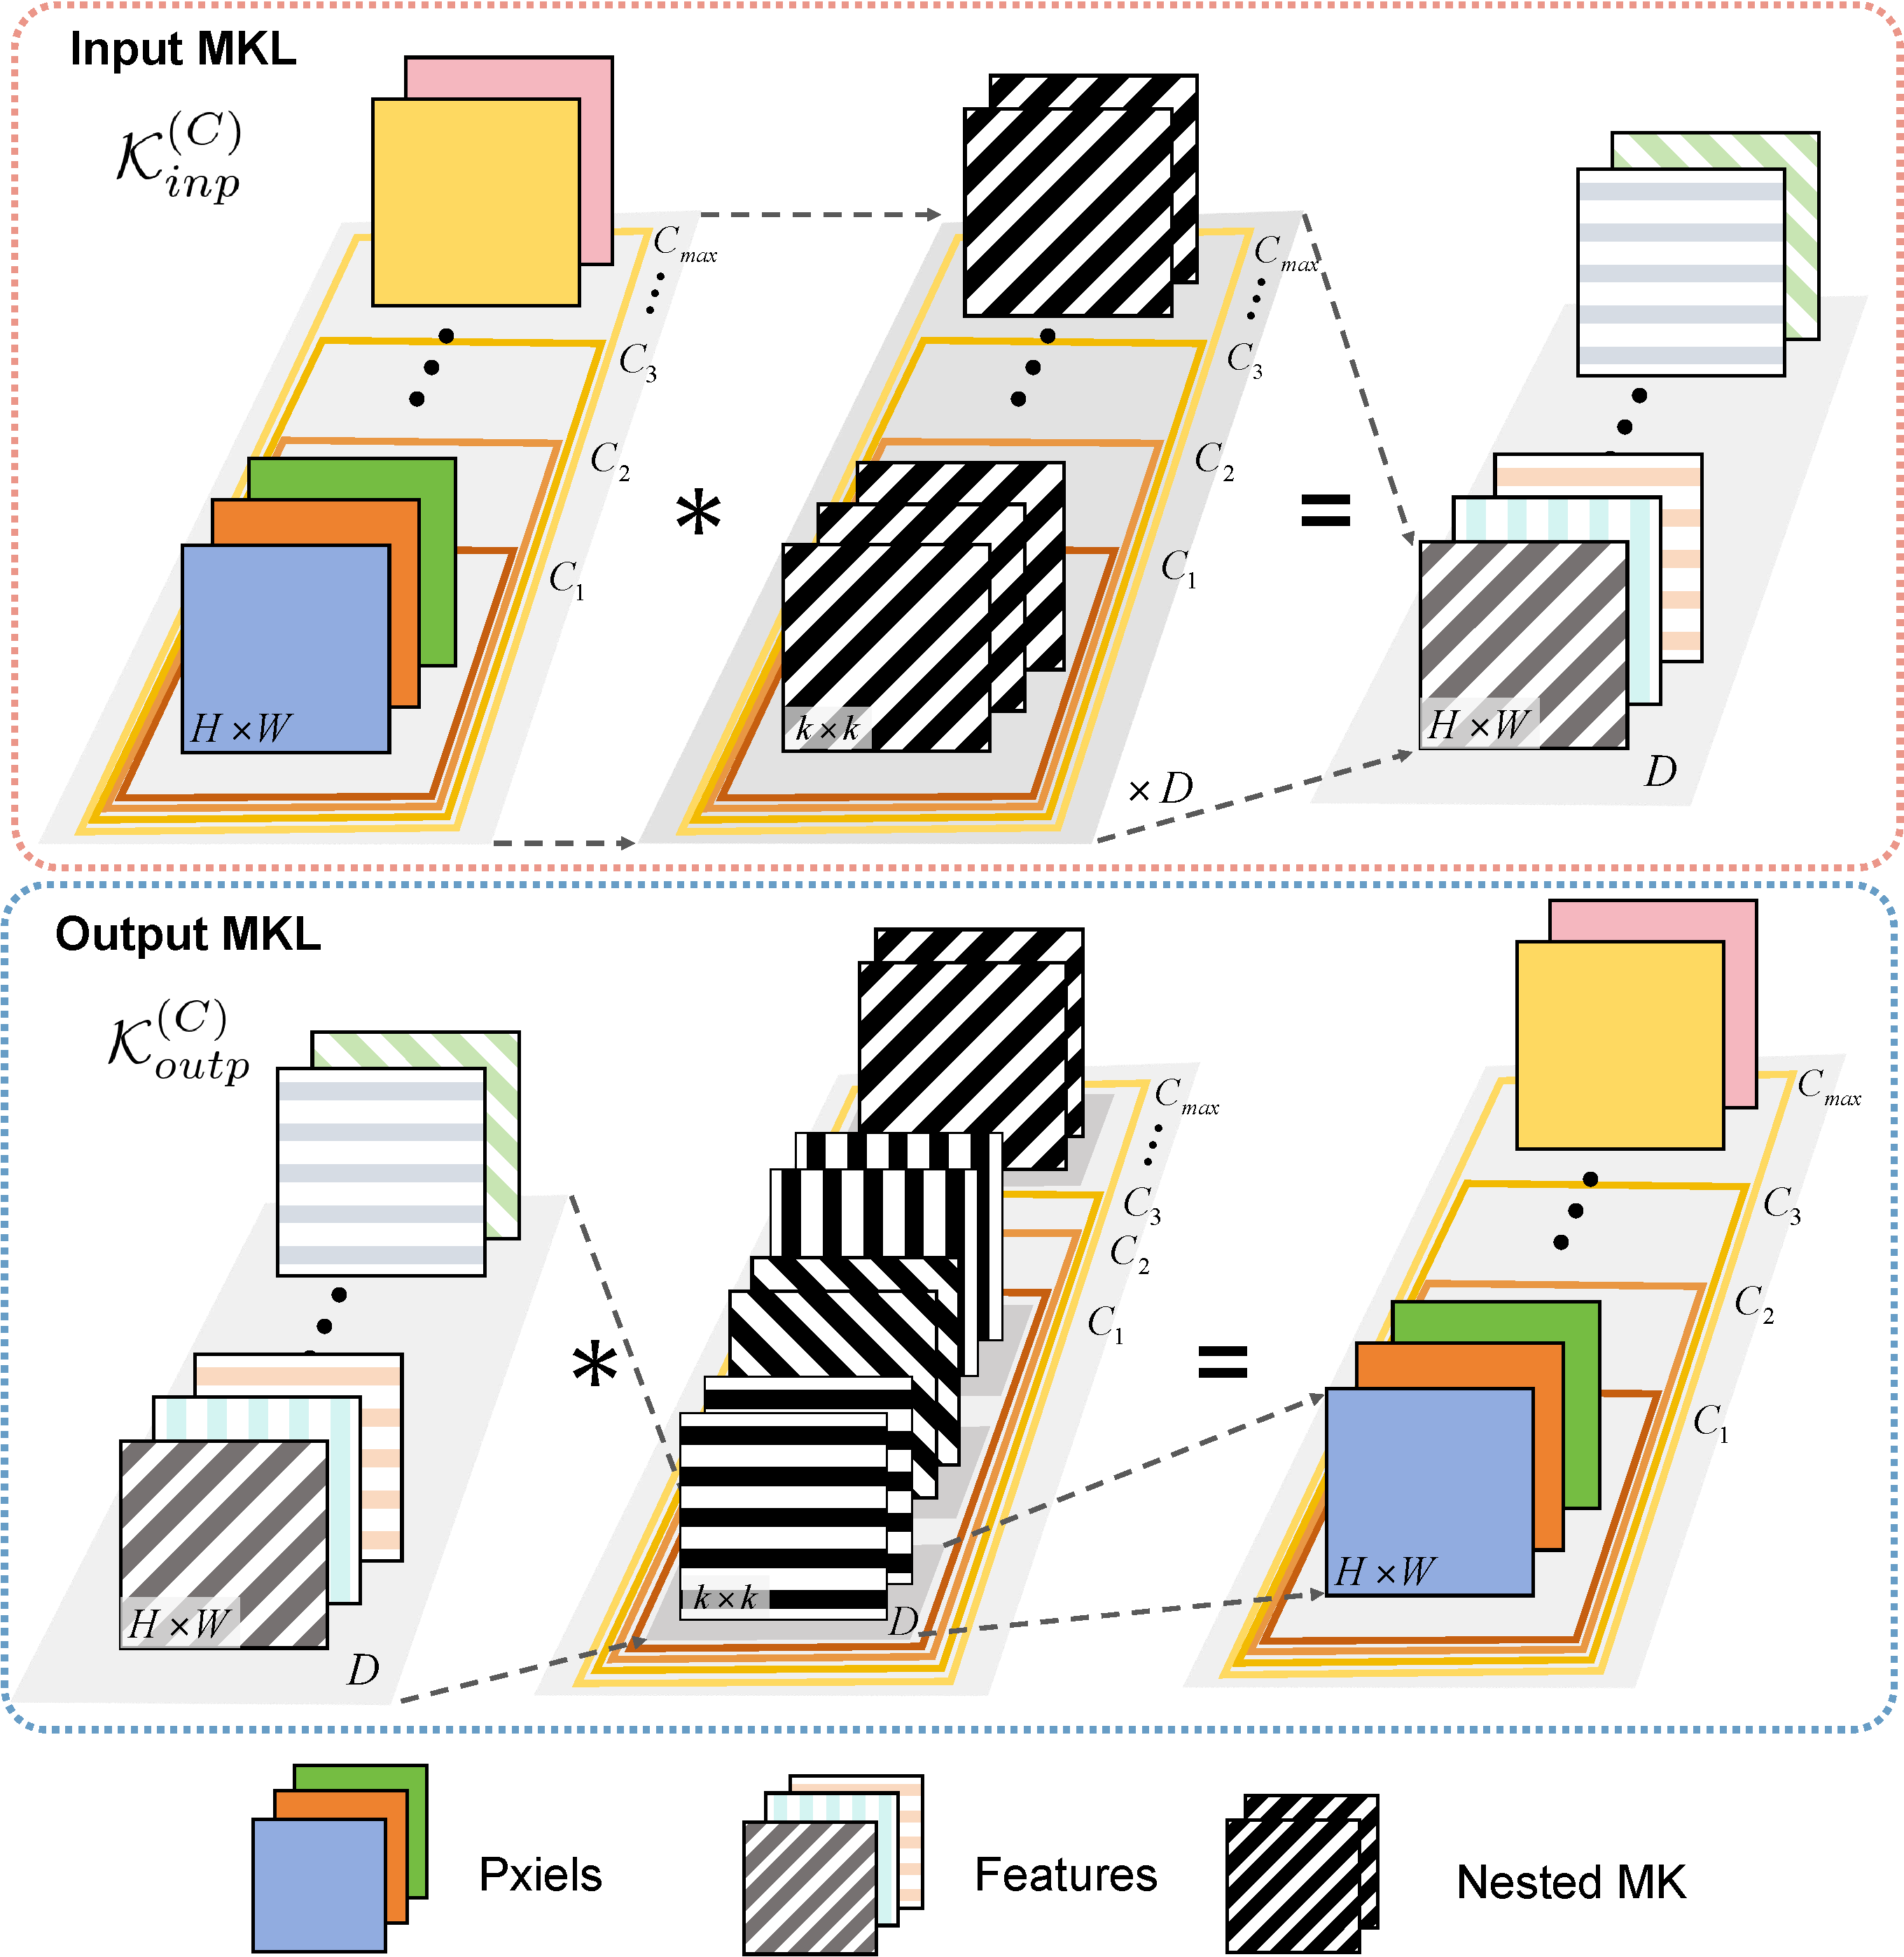
\includegraphics[width=\linewidth]{Figs/mk-2.pdf}
    \caption{Illustration of the MKL's encoding and decoding.}
    \label{fig:placeholder}
\end{figure}
% In a standard convolutional layer, its weight tensor $\mathbf{W}$ has a shape of $(C_{out}, C_{in}, k, k)$, where the input channel dimension $C_{in}$ is fixed upon model initialization. This hard-coded design inextricably ties a standard model to the spectral band count of a specific sensor, rendering it incapable of directly processing data from other sensors with a different $C_{in}$.

% To break this limitation, our Spectral-Agnostic Layers, upon initialization, does not create a kernel for a specific $C_{in}$ but rather a ``superset'' kernel designed with a capacity far exceeding that of any single dataset. The weight tensor of this kernel, $\mathbf{W}_{super}$, has a shape of $(C_{out}, C_{max}, k, k)$, where $C_{max}$ is a predefined maximum channel capacity (e.g., 200) sufficient to accommodate all potential inputs. This ``superset'' kernel conceptually contains all the smaller ``subset'' kernels that might be needed. For instance, a kernel designed to process 31-channel data can be considered a subset of this 200-channel ``superset'' kernel.

% During the forward pass, the layer does not use the entire ``superset'' kernel. Instead, it dynamically and non-parametrically ``slices'' a perfectly matched ``subset'' kernel, $\mathbf{W}_{sub}$, based on the actual channel count $C$ of the input tensor $\mathcal{Y}$ (i.e., the third dimension of $\mathcal{Y}$). This operation can be formally expressed as:
% \begin{equation}
%     \mathbf{W}_{sub} = \mathbf{W}_{super}[:, :C, :, :]
%     \label{eq:slicing}
% \end{equation}
% Subsequently, only this sliced ``subset'' kernel $\mathbf{W}_{sub}$ is used for the actual convolution operation:
% \begin{equation}
%     \text{Output} = \text{Conv}(\mathcal{Y}, \mathbf{W}_{sub}, b)
% \end{equation}

A similar nested philosophy is applied to the output MKL of the model, enabling it to dynamically generate an output that matches the original band count $C$ of the input sample.
During the forward pass, a desired output channel count, $C_{\text{out}}$ ($C_{\text{out}} \le C_{\text{max}}$), is specified. The valid kernel $\mathbf{W}_{\text{valid}} \in \mathbb{R}^{C_{\text{out}} \times D \times k \times k}$ and bias $\mathbf{b}_{\text{comp}} \in \mathbb{R}^{C_{\text{out}}}$ are generated by slicing the superset parameters along the output channel dimension:
\begin{align}
    \mathbf{W}_{\text{valid}} &= \mathbf{W}_{\text{nested}}[:C_{\text{out}}, :, :, :], \\
    \mathbf{b}_{\text{valid}} &= \mathbf{b}_{\text{nested}}[:C_{\text{out}}].
    \label{eq:output_slice_w}
\end{align}
Through this mechanism of a nested kernel and dynamic subset slicing, our SSA model achieves true spectral agnosticism, allowing it to seamlessly process heterogeneous data from any sensor within a universal architecture. The detailed input and output MKL algorithms are shown in App.\S~\ref{mkl_algos}.

% % Define custom colors for highlighting
% \definecolor{bestcolor}{RGB}{255, 224, 224}
% \definecolor{secondcolor}{RGB}{224, 224, 255}
% \definecolor{normalcolor}{RGB}{255, 255, 255} % White for normal cells

% % --- NEW COMMANDS FOR SINGLE-CELL RENDERING ---
% % This command creates a perfectly aligned value ± std pair in a single cell
% % It uses an inner tabular to achieve alignment on the ± symbol
% \newcommand{\perfalign}[3]{% #1: value, #2: symbol, #3: std
%     \begin{tabular}{@{}r@{\,}l@{}}
%         #1 & #2\ #3
%     \end{tabular}
% }
% \newcommand{\perfalignplain}[2]{% #1: value, #2: std (for DCFormer)
%     \begin{tabular}{@{}r@{\ }l@{}}
%         #1 & #2
%     \end{tabular}
% }

% % Commands to apply background color to a SINGLE CELL
% \newcommand{\best}[1]{\cellcolor{bestcolor}\perfalign{#1}}
% \renewcommand{\second}[1]{\cellcolor{secondcolor}\perfalign{#1}}
% \newcommand{\normal}[1]{\cellcolor{normalcolor}\perfalign{#1}}
% \newcommand{\bestplain}[1]{\cellcolor{bestcolor}\perfalignplain{#1}}
% \newcommand{\secondplain}[1]{\cellcolor{secondcolor}\perfalignplain{#1}}


\begin{table*}[!ht]
\centering
\renewcommand{\arraystretch}{1.0}
\setlength{\tabcolsep}{1pt}
\caption{The average and standard deviation calculated for all the compared approaches on 10 CAVE examples and 2 the PaviaC dataset examples simulating $\times4$ (in-distribution) and $\times 8,\times 16,\times 32$ (\textit{out-of-distribution}). Results are highlighted as 
    \colorbox{bestcolor}{best} and \colorbox{secondcolor}{second best}.}
\label{tab:cave_pavia_quantitative_comparison}
% \sisetup{}

\resizebox{\textwidth}{!}{%
% Each model now uses a single centered 'c' column
\begin{tabular}{@{}l l l 
  c c c c c c c | c c c c c c c @{}}
\toprule
\midrule
\multicolumn{3}{c}{\multirow{2}{*}{\textbf{Metric}}} & \multicolumn{7}{c}{\textbf{CAVE Dataset}} & \multicolumn{7}{c}{\textbf{PaviaC Dataset}} \\

\cmidrule(lr){4-10} \cmidrule(l){11-17}
\multicolumn{3}{c}{} 
& \textbf{DSPNet} & \textbf{MIMO-SST} & \textbf{DCINN} & \textbf{DCFormer} & \textbf{PSTUN} & \textbf{LRTN} & \textbf{Ours}
& \textbf{DSPNet} & \textbf{MIMO-SST} & \textbf{DCINN} & \textbf{DCFormer} & \textbf{PSTUN} & \textbf{LRTN} & \textbf{Ours} \\
\midrule
% --- 4× In-Dist. 数据行 ---
\multirow{4}{*}{\rotatebox[origin=c]{90}{In-Dist.}} & \multirow{4}{*}{$\times$4}
& PSNR($\uparrow$) 
& \normal{40.37}{$\pm$}{3.25} & \normal{45.35}{$\pm$}{3.35} & \normal{43.75}{$\pm$}{3.77} & \secondplain{45.81}{$\pm$}{5.56} & \normal{40.57}{$\pm$}{3.72} & \normal{41.13}{$\pm$}{3.24} & \best{45.96}{$\pm$}{4.69}
& \normal{43.89}{$\pm$}{1.78} & \normal{42.04}{$\pm$}{0.78} & \normal{44.79}{$\pm$}{1.99} & \normal{42.61}{$\pm$}{1.19} & \normal{44.94}{$\pm$}{1.50} & \secondd{45.13}{$\pm$}{1.01} & \best{45.92}{$\pm$}{1.75} \\
& & SAM($\downarrow$) 
& \normal{2.72}{$\pm$}{0.89} & \normal{2.74}{$\pm$}{0.86} & \normal{2.72}{$\pm$}{0.81} & \secondplain{2.70}{$\pm$}{1.03} & \normal{2.94}{$\pm$}{0.89} & \normal{2.92}{$\pm$}{1.38} & \best{2.55}{$\pm$}{1.00}
& \normal{3.15}{$\pm$}{0.43} & \normal{3.29}{$\pm$}{0.45} & \secondd{2.59}{$\pm$}{0.41} & \normal{3.55}{$\pm$}{0.43} & \normal{2.95}{$\pm$}{0.46} & \normal{3.18}{$\pm$}{0.45} & \best{2.02}{$\pm$}{0.30} \\
& & ERGAS($\downarrow$) 
& \normal{2.51}{$\pm$}{0.71} & \normal{2.08}{$\pm$}{0.68} & \normal{2.37}{$\pm$}{0.95} & \secondplain{2.01}{$\pm$}{1.82} & \normal{2.70}{$\pm$}{0.89} & \normal{2.38}{$\pm$}{0.82} & \best{1.72}{$\pm$}{1.13}
& \normal{1.58}{$\pm$}{0.10} & \normal{1.73}{$\pm$}{0.02} & \normal{1.34}{$\pm$}{0.12} & \normal{1.82}{$\pm$}{0.05} & \normal{1.47}{$\pm$}{0.07} & \normal{1.48}{$\pm$}{0.01} & \best{1.07}{$\pm$}{0.11} \\
& & SSIM($\uparrow$) 
& \normal{0.993}{$\pm$}{0.005} & \best{0.994}{$\pm$}{0.005} & \normal{0.992}{$\pm$}{0.004} & \secondplain{0.993}{$\pm$}{0.004} & \normal{0.992}{$\pm$}{0.005} & \normal{0.992}{$\pm$}{0.006} & \best{0.994}{$\pm$}{0.005}
& \normal{0.988}{$\pm$}{0.000} & \normal{0.986}{$\pm$}{0.000} & \secondd{0.992}{$\pm$}{0.000} & \normal{0.983}{$\pm$}{0.000} & \normal{0.990}{$\pm$}{0.000} & \normal{0.988}{$\pm$}{0.000} & \best{0.996}{$\pm$}{0.000} \\
\cmidrule(lr){1-17}
% --- 8× Out-of-Dist. 数据行 ---
\multirow{12}{*}{\rotatebox[origin=c]{90}{Out-of-Dist.}} & \multirow{4}{*}{$\times$8}
& PSNR($\uparrow$) 
& \normal{36.92}{$\pm$}{3.47} & \normal{29.73}{$\pm$}{3.21} & \normal{33.72}{$\pm$}{3.39} & \bestplain{41.46}{$\pm$}{4.98} & \normal{34.69}{$\pm$}{3.17} & \normal{33.40}{$\pm$}{3.13} & \secondd{38.80}{$\pm$}{3.79}
& \normal{38.03}{$\pm$}{0.80} & \normal{34.45}{$\pm$}{0.55} & \normal{32.82}{$\pm$}{0.58} & \normal{36.57}{$\pm$}{0.88} & \secondd{37.27}{$\pm$}{0.93} & \normal{33.57}{$\pm$}{0.40} & \best{38.59}{$\pm$}{0.67} \\
& & SAM($\downarrow$) 
& \normal{3.82}{$\pm$}{1.59} & \normal{5.55}{$\pm$}{2.66} & \normal{4.33}{$\pm$}{1.94} & \bestplain{3.65}{$\pm$}{1.65} & \normal{4.30}{$\pm$}{1.59} & \normal{4.55}{$\pm$}{2.03} & \secondd{3.70}{$\pm$}{1.45}
& \normal{5.66}{$\pm$}{0.25} & \normal{6.70}{$\pm$}{0.14} & \normal{6.09}{$\pm$}{0.19} & \secondd{5.49}{$\pm$}{0.26} & \normal{5.48}{$\pm$}{0.20} & \normal{6.67}{$\pm$}{0.15} & \best{4.74}{$\pm$}{0.06} \\
& & ERGAS($\downarrow$) 
& \normal{3.91}{$\pm$}{1.44} & \normal{9.91}{$\pm$}{4.03} & \normal{6.24}{$\pm$}{2.62} & \bestplain{3.08}{$\pm$}{2.21} & \normal{5.13}{$\pm$}{1.93} & \normal{6.00}{$\pm$}{2.03} & \secondd{3.46}{$\pm$}{1.57}
& \normal{4.05}{$\pm$}{0.05} & \normal{4.53}{$\pm$}{0.07} & \normal{4.53}{$\pm$}{0.09} & \normal{3.79}{$\pm$}{0.06} & \secondd{3.60}{$\pm$}{0.06} & \normal{4.51}{$\pm$}{0.05} & \best{3.47}{$\pm$}{0.05} \\
& & SSIM($\uparrow$) 
& \normal{0.980}{$\pm$}{0.015} & \normal{0.904}{$\pm$}{0.099} & \normal{0.958}{$\pm$}{0.029} & \bestplain{0.985}{$\pm$}{0.014} & \normal{0.964}{$\pm$}{0.022} & \normal{0.956}{$\pm$}{0.030} & \secondd{0.982}{$\pm$}{0.013}
& \normal{0.947}{$\pm$}{0.004} & \normal{0.923}{$\pm$}{0.006} & \normal{0.929}{$\pm$}{0.005} & \normal{0.948}{$\pm$}{0.004} & \normal{0.953}{$\pm$}{0.003} & \normal{0.931}{$\pm$}{0.006} & \best{0.960}{$\pm$}{0.004} \\
\cmidrule(lr){2-17}
% --- 16× Out-of-Dist. 数据行 ---
& \multirow{4}{*}{$\times$16}
& PSNR($\uparrow$) 
& \secondd{30.87}{$\pm$}{3.46} & \normal{24.76}{$\pm$}{2.93} & \normal{27.65}{$\pm$}{3.43} & - & \normal{29.47}{$\pm$}{3.16} & \normal{27.53}{$\pm$}{2.97} & \best{31.84}{$\pm$}{3.47}
& \normal{32.92}{$\pm$}{0.43} & \normal{31.49}{$\pm$}{0.20} & \normal{28.74}{$\pm$}{0.05} & - & \secondd{34.28}{$\pm$}{0.39} & \normal{28.65}{$\pm$}{0.11} & \best{35.00}{$\pm$}{0.02} \\
& & SAM($\downarrow$) 
& \secondd{6.51}{$\pm$}{2.83} & \normal{8.36}{$\pm$}{4.48} & \normal{6.93}{$\pm$}{3.48} & - & \normal{6.68}{$\pm$}{2.44} & \normal{6.73}{$\pm$}{3.08} & \best{5.93}{$\pm$}{2.42}
& \normal{8.43}{$\pm$}{0.39} & \normal{8.94}{$\pm$}{0.13} & \normal{8.72}{$\pm$}{0.18} & - & \secondd{7.48}{$\pm$}{0.30} & \normal{9.64}{$\pm$}{0.10} & \best{6.89}{$\pm$}{0.08} \\
& & ERGAS($\downarrow$) 
& \secondd{7.58}{$\pm$}{2.66} & \normal{16.69}{$\pm$}{6.56} & \normal{12.19}{$\pm$}{4.99} & - & \normal{8.85}{$\pm$}{2.80} & \normal{11.44}{$\pm$}{4.40} & \best{7.30}{$\pm$}{2.88}
& \normal{6.79}{$\pm$}{0.05} & \normal{6.25}{$\pm$}{0.07} & \normal{6.78}{$\pm$}{0.17} & - & \best{5.04}{$\pm$}{0.04} & \normal{7.39}{$\pm$}{0.30} & \secondd{5.16}{$\pm$}{0.07} \\
& & SSIM($\uparrow$) 
& \secondd{0.947}{$\pm$}{0.032} & \normal{0.834}{$\pm$}{0.102} & \normal{0.901}{$\pm$}{0.061} & - & \normal{0.926}{$\pm$}{0.037} & \normal{0.905}{$\pm$}{0.057} & \best{0.953}{$\pm$}{0.029}
& \normal{0.910}{$\pm$}{0.001} & \normal{0.898}{$\pm$}{0.003} & \normal{0.880}{$\pm$}{0.002} & - & \secondd{0.932}{$\pm$}{0.001} & \normal{0.883}{$\pm$}{0.005} & \best{0.935}{$\pm$}{0.002} \\
\cmidrule(lr){2-17}
% --- 32× Out-of-Dist. 数据行 ---
& \multirow{4}{*}{$\times$32}
& PSNR($\uparrow$) 
& \secondd{27.91}{$\pm$}{2.95} & \normal{21.85}{$\pm$}{2.56} & \normal{23.96}{$\pm$}{2.77} & - & \normal{27.55}{$\pm$}{2.75} & \normal{24.48}{$\pm$}{2.69} & \best{28.06}{$\pm$}{2.64}
& \normal{30.51}{$\pm$}{0.21} & \normal{29.91}{$\pm$}{0.02} & \normal{26.51}{$\pm$}{0.17} & - & \secondd{32.63}{$\pm$}{0.46} & \normal{26.53}{$\pm$}{0.41} & \best{32.79}{$\pm$}{0.26} \\
& & SAM($\downarrow$) 
& \normal{10.03}{$\pm$}{3.94} & \normal{12.26}{$\pm$}{5.90} & \normal{10.34}{$\pm$}{4.73} & - & \secondd{9.43}{$\pm$}{3.28} & \normal{9.64}{$\pm$}{3.96} & \best{8.64}{$\pm$}{3.17}
& \normal{10.26}{$\pm$}{0.51} & \normal{10.69}{$\pm$}{0.33} & \normal{10.93}{$\pm$}{0.47} & - & \secondd{9.16}{$\pm$}{0.66} & \normal{11.89}{$\pm$}{0.43} & \best{8.49}{$\pm$}{0.19} \\
& & ERGAS($\downarrow$) 
& \best{11.12}{$\pm$}{3.90} & \normal{23.54}{$\pm$}{8.22} & \normal{18.98}{$\pm$}{4.18} & - & \normal{12.35}{$\pm$}{3.30} & \normal{16.80}{$\pm$}{5.97} & \secondd{11.40}{$\pm$}{6.69}
& \normal{8.62}{$\pm$}{0.57} & \normal{7.39}{$\pm$}{0.33} & \normal{8.44}{$\pm$}{0.50} & - & \best{6.00}{$\pm$}{0.32} & \normal{9.26}{$\pm$}{0.85} & \secondd{6.24}{$\pm$}{0.30} \\
& & SSIM($\uparrow$) 
& \secondd{0.912}{$\pm$}{0.036} & \normal{0.774}{$\pm$}{0.099} & \normal{0.843}{$\pm$}{0.066} & - & \normal{0.896}{$\pm$}{0.034} & \normal{0.860}{$\pm$}{0.061} & \best{0.918}{$\pm$}{0.032}
& \normal{0.893}{$\pm$}{0.002} & \normal{0.887}{$\pm$}{0.000} & \normal{0.853}{$\pm$}{0.003} & - & \secondd{0.919}{$\pm$}{0.004} & \normal{0.856}{$\pm$}{0.001} & \best{0.922}{$\pm$}{0.001} \\
\midrule
\bottomrule
\end{tabular}%
}
\vspace{-1em}
\end{table*}
\subsection{Arbitrary-Scale Image Fusion as Continuous Function}
\label{subsec:inr}
The implementation of our target HR-HSI as a continuous function through the implicit fusion backbone $\Gamma$ is what grants our model true spatial flexibility. It allows the model to be queried on any coordinate grid, enabling the generation of an output at any desired resolution.

As illustrated in Fig.~\ref{fig: architecture} (b), our model first maps the embedded features after MK into a latent space via two parallel encoders $ \phi_\alpha,  \psi_\beta$. This process can be represented as:
\begin{equation}
\begin{cases} 
\mathcal E_{pe} = \phi_{\alpha}(\mathcal K_{inp}^{(C)}(\ylr)), \\
\mathcal{E}_{pa} = \psi_{\beta}\left(\mathcal K_{inp}^{(C)}([\mathcal{Y}_{HR}; \mathcal{Z}_{HR}])\right), \notag
\end{cases}
\end{equation}
where $[\cdot;\cdot]$ stands for channel concatenation. These latent codes, $\mathcal{E}_{pe}$ and $\mathcal{E}_{pa}$, provide both the spectral and spatial semantic information necessary for the subsequent continuous function modeling.

To predict the spectral vector for any continuous coordinate $\mathbf{p}$ in the target HR-HSI space, our fusion module performs a local, query-based process. For a given pixel, we use its center to represent its coordinate and map the HR coordinates to a normalized square grid $\Omega = [-1,1]^2$. The integer coordinates $(i,j)$ of a pixel in the $H\times W$ source grid are then mapped to a query coordinate $\mathbf p_{(i,j)}\in \Omega \subset \mathbb R^2$ using the following transformation:
\begin{equation}
    \mathbf{p}_{(i,j)} = \left( \frac{2i}{H-1} - 1, \frac{2j}{W-1} - 1 \right).
\end{equation}
Using the query coordinate $\mathbf{p}$ as a pivot, we sample a precise local spatial feature from the spatial latent code $\mathcal{E}_{pa}$. Concurrently, we identify the nearest neighbor $\mathbf{q}_{(i,j)}\in \Omega$ corresponding to $\mathbf{p}_{(i,j)}$ in the low-resolution spectral latent code $\mathcal{E}_{pe}$ and sample the features of this neighbor.

For the sampled local spectral features, we feed the previous spectral, spatial codes and the relative coordinates $\mathbf{p}-\mathbf{q}$ that describe the fine-grained position into a shared MLP decoder:
\begin{equation}
    \widehat{\mathcal{X}}^{res}(\mathbf{p}) = \texttt{MLP}(\mathcal{E}_{pe}(\mathbf{p}), \mathcal{E}_{pa}(\mathbf{q}), \mathbf{p}-\mathbf{q}),
\end{equation}
where $\mathbf{p}$ is the normalized coordinates of each query pixel in the HR domain. The output of the MLP is then fed into the output MK layer. Leveraging the MK, this layer dynamically maps the MLP feature back to the original spectral band count $C$ of the current sample, generating the final predicted residual components $\mathcal K_{outp}^{(C)}(\widehat{\mathcal{X}}^{res}(\mathbf{p}))$. The complete fused image is finally obtained by adding the predicted residual to the bicubic-interpolated base image:
\begin{equation}
    \widehat{\mathcal{X}}_{HR}(\mathbf{p}) = \mathcal{Y}_{HR}(\mathbf{p}) + \mathcal K_{outp}^{(C)}(\widehat{\mathcal{X}}^{res}(\mathbf{p})).
\end{equation}

Additionally, to ensure spatial continuity when crossing grid boundaries, we follow the practice of LIIF~\cite{chen2021learning}. We identify the four-nearest neighbor grid points $\mathbf q_{i}, i\in \{1,\dots 4\}
$ in the low-resolution feature map. During decoding, we predict a candidate spectral residual $\widehat{\mathcal{X}}^{res}_i(\mathbf{p})$ and a scalar weight $w_i$ for each neighbor $q_i$. The final residual vector is then obtained by a softmax weighted fusion of all candidate residuals:
\begin{equation}
    \widehat{\mathcal{X}}^{res}(\mathbf{p}) = \sum_{i=1}^4 \frac{\exp(w_i)}{\sum_{j=1}^4 \exp(w_j)} \widehat{\mathcal{X}}^{res}_i(\mathbf{p}).
\end{equation}
True scale agnosticism is achieved through this coordinate-based approach. By modeling the HR-HSI as a continuous function, our architecture avoids fixed upsampling layers, granting it the ability to generate outputs at any resolution.
\begin{figure*}[!ht]
    \centering
    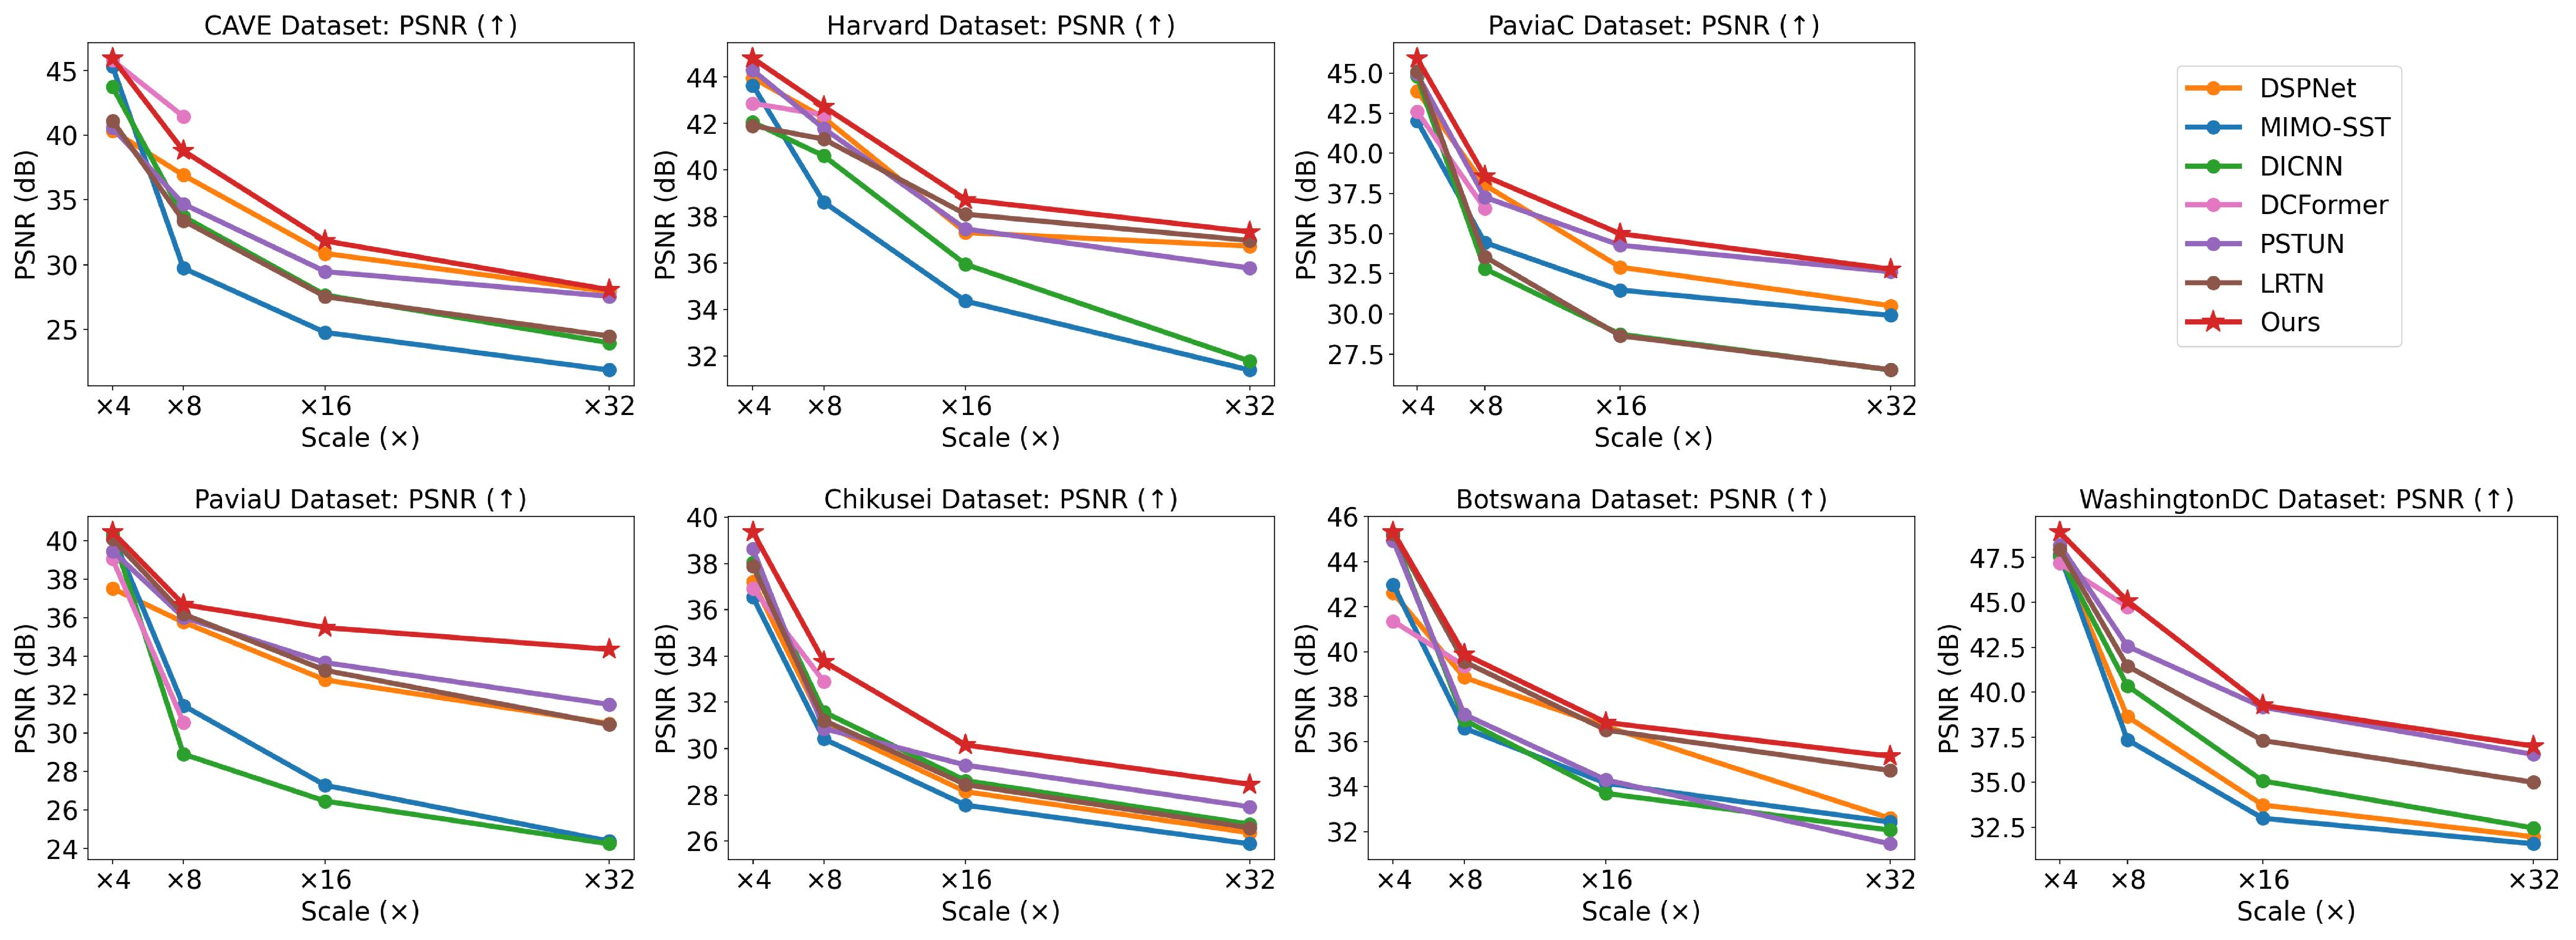
\includegraphics[width=\textwidth]{Figs/psnr.pdf}
    \caption{Quantitative comparison of PSNR (dB) across multiple scaling factors on all seven datasets.}
    \label{fig:psnr}
\end{figure*}
\subsection{Cross-Sensor Joint Training Strategy}
\label{subsec:training}

The conventional ``one dataset, one model'' paradigm is not only inefficient but also prone to being easily overfitting~\cite{yan2025hyperspectral}, especially given the small scale of HSI datasets. Training a universal model within various hyperspectral data usually faces a challenge that different bands and spatial sizes can not be batched together to enable joint training.

Our training pipeline is designed to handle $N$ heterogeneous datasets, denoted as $\mathcal{D} = \{D_1, \dots, D_N\}$.
We first partition all training samples into distinct buckets, where each bucket  $D_i$ contains data from a single source dataset, thus sharing identical spatial dimensions and number of spectral bands. 
At each training step, we construct a mini-batch by a two-stage sampling process. First, a bucket $D_i$ is selected from $\mathcal D$ following a uniform random distribution. Then, a batch of samples is drawn exclusively from the chosen bucket. This strategy ensures that all samples within a single mini-batch are structurally homogeneous, while samples across different mini-batches can be heterogeneous.
It is precisely this batch-to-batch heterogeneity that our model is designed for.
% Thanks to our Matryoshka Kernels (\S\ref{subsec:mk}) and Continuous Representation (\S\ref{subsec:inr}), the model seamlessly adapts to the structural differences from one batch to the next. 
Crucially, all samples are processed by a universal model parameters $\theta$, which are optimized via a unified hybrid reconstruction loss function.
Following Eq.~\eqref{eq:mrl-loss}, the reconstruction loss can be written in the MRL style:
\begin{equation}
    \min_{\substack{\theta,\, C\in \text{Dim}(D_i), \\ (\ylr,\zhr)\in D_i}} \frac 1 N \sum_{i=1}^N  \mathcal L_{total}\left[ \mathcal F_\theta( \ylr,\zhr); \xhr \right],  \notag 
\end{equation}
where $\mathcal F_\theta$ is the model (\textit{i.e.}, $\mathcal F_\theta:=\mathcal K_{outp}^{(C)} \circ \Gamma \circ \mathcal K_{inp}^{(C)}$ and $\circ$ means the network composition), Dim$(\cdot)$  denotes the bands numbers in the data bucket. Our total loss, $\mathcal{L}_{total}$, is a weighted sum of the L1 loss and the Structural Similarity (SSIM) loss, defined as:
\begin{equation}
\begin{aligned}
    &\mathcal{L}_{total} = \mathbb{E}_{(\mathcal{Y}_{LR}, \mathcal{Z}_{HR}, \mathcal{X}_{HR}) \sim D_{i}} \left[ \mathcal{L}_{1}+ \lambda\mathcal{L}_{SSIM} \right], \\
    &\mathcal{L}_{1} = \| \mathcal{F}_\theta(\mathcal{Y}_{LR}, \mathcal{Z}_{HR})  - \mathcal{X}_{HR} \|_1 ,\\
    &\mathcal{L}_{SSIM} = 1 - \text{SSIM}(\mathcal{F}_\theta(\mathcal{Y}_{LR}, \mathcal{Z}_{HR}), \mathcal{X}_{HR}),
\end{aligned}
\end{equation}
where $\lambda$ is a weighting coefficient, $\| \cdot \|$ is the $\ell_1$ norm, and $\text{SSIM}(\cdot, \cdot)$ is the structural similarity index measure.

Through this joint training strategy, our SSA model is forced to learn a universal fusion mapping rather than memorizing the specifics of a particular dataset.
This approach endows the model with remarkable generalization capabilities to unseen sensors (see \S~\ref{sec:generalization}).
